\section{非周期信号的频谱}

\subsection{傅里叶变换}

\begin{BoxDefinition}[傅里叶变换]*
    $f(t)$的傅里叶变换
    \begin{Equation}
        F(\mathrm{j}\omega)=\int_{-\infty}^{\infty}f(t)e^{-\mathrm{j}\omega t}dt
    \end{Equation}
    简记为
    \begin{Equation}
        F(\mathrm{j}\omega)=\mathscr{F}\left[f(t)\right]
    \end{Equation}

    $F(\mathrm{j}\omega)$的傅里叶逆变换
    \begin{Equation}
        f(t)=\frac{1}{2\pi}\int_{-\infty}^{\infty}F(\mathrm{j}\omega)e^{\mathrm{j}\omega t}d\omega
    \end{Equation}
    简记为
    \begin{Equation}
        f(t)=\mathscr{F}^{-1}\left[F(\mathrm{j}\omega)\right]
    \end{Equation}
    $F(\mathrm{j}\omega)$一般是复函数,写为
    \begin{Equation}
        F(\mathrm{j}\omega) = |F(\mathrm{j}\omega)|e^{\mathrm{j}\varphi(\omega)}=R(\omega)+\mathrm{j}X(\omega)
    \end{Equation}
    傅里叶变换存在的充分条件
    \begin{Equation}
        \int_{-\infty}^{\infty}|f(t)|dt<\infty
    \end{Equation}
    运用下列关系可以方便计算一些积分
    \begin{Equation}
        f(0) = \frac{1}{2\pi}\int_{-\infty}^{\infty}F(\mathrm{j}\omega)d\omega
    \end{Equation}
    \begin{Equation}
        F(0) = \int_{-\infty}^{\infty}f(t)dt
    \end{Equation}
\end{BoxDefinition}

\subsection{常用函数的傅里叶变换}

\begin{BoxFormula}[门函数的傅里叶变换]*
    门函数记为$g_{\tau}(t)$
    \begin{Figure}[门函数]
        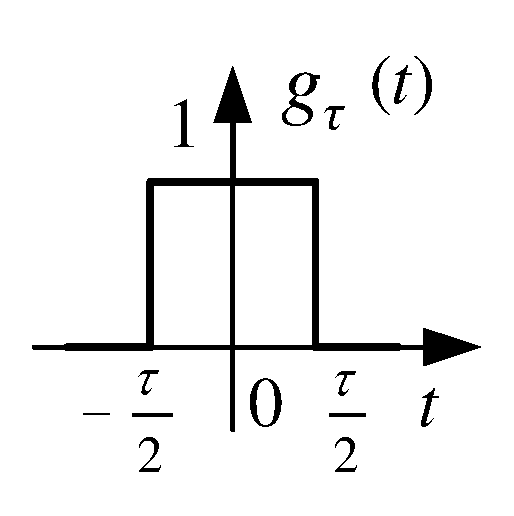
\includegraphics[width=15mm]{visio/4.7.pdf}
    \end{Figure}
    其傅里叶变换为
    \begin{Equation}
        F(\mathrm{j}\omega) = \int_{-\frac{\tau}{2}}^{\frac{\tau}{2}}e^{-\mathrm{j}\omega t}dt = \tau\cdot\mathrm{Sa}(\frac{\omega\tau}{2})
    \end{Equation}
\end{BoxFormula}

当频谱函数为实函数或虚函数时,只需要幅度频谱函数$|F(\mathrm{j}\omega)|$即可表示整个频谱函数,否则还需要相位频谱函数$\varphi(\omega)$。
\begin{BoxFormula}[单边指数函数的傅里叶变换]
    单边指数函数
    \begin{Equation}
        f(t)=e^{-\alpha t}\varepsilon(t) \ (\alpha > 0)
    \end{Equation}
    傅里叶变换
    \begin{Equation}
        \begin{aligned}
            F(\mathrm{j}\omega) & = \int_{-\infty}^{\infty}f(t)e^{-\mathrm{j}\omega t}dt                \\
                                & = \int_{0}^{\infty} e^{-(\alpha+\mathrm{j}\omega)t}dt                 \\
                                & = \frac{1}{\alpha+\mathrm{j}\omega}                                   \\
                                & = \frac{1}{\sqrt{\alpha^2+\omega^2}}e^{-\arctan\frac{\omega}{\alpha}}
        \end{aligned}
    \end{Equation}
    即
    \begin{Figure}[单边指数函数的频谱函数图像]
        \begin{FigureSub}[单边指数函数的幅度频谱]
            \quad\quad
            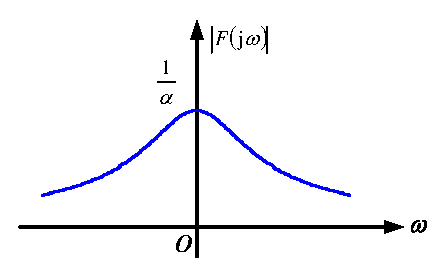
\includegraphics[width=30mm]{visio/4.8-a.pdf}
            \quad\quad
        \end{FigureSub}
        \begin{FigureSub}[单边指数函数的相位频谱]
            \quad\quad
            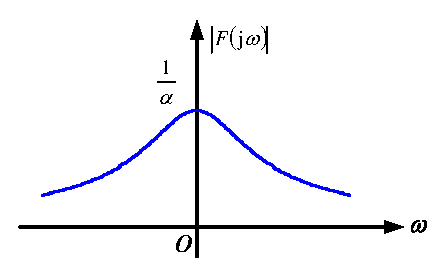
\includegraphics[width=30mm]{visio/4.8-a.pdf}
            \quad\quad
        \end{FigureSub}
    \end{Figure}
    \begin{Equation}
        |F(\mathrm{j}\omega)| = \frac{1}{\sqrt{\alpha^2+\omega^2}},\ \varphi(t) = -\arctan\frac{\omega}{\alpha}
    \end{Equation}
\end{BoxFormula}

\begin{BoxFormula}[双边指数函数的傅里叶变换]
    双边指数函数
    \begin{Equation}
        f(t) = e^{-\alpha|t|} \ (\alpha > 0)
    \end{Equation}
    傅里叶变换
    \begin{Equation}
        \begin{aligned}
            F(\mathrm{j}\omega) & = \int_{-\infty}^{\infty}f(t)e^{-\mathrm{j}\omega t}dt                                             \\
                                & = \int_{-\infty}^{0}f(t)e^{-\mathrm{j}\omega t}dt + \int_{0}^{\infty}f(t)e^{-\mathrm{j}\omega t}dt \\
                                & = \frac{1}{\alpha-\mathrm{j}\omega} + \frac{1}{\alpha+\mathrm{j}\omega}                            \\
                                & = \frac{2\alpha}{\alpha^2+\omega^2}
        \end{aligned}
    \end{Equation}
    \begin{Figure}[双边指数函数的频谱函数图像]
        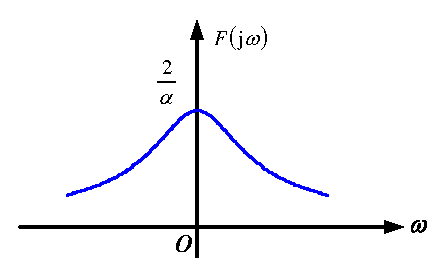
\includegraphics[width=30mm]{visio/4.9.pdf}
    \end{Figure}
    \ 
\end{BoxFormula}

\begin{BoxFormula}[冲激函数的傅里叶变换]
    对于冲激函数$\delta(t)$,其傅里叶变换为
    \begin{Equation}
        F(\mathrm{j}\omega) = \int_{-\infty}^{\infty}\delta(t)e^{-\mathrm{j}\omega t }dt = 1
    \end{Equation}
    对于冲激偶$\delta'(t)$,其傅里叶变换为
    \begin{Equation}
        F(\mathrm{j}\omega) = \int_{-\infty}^{\infty}\delta'(t)e^{-\mathrm{j}\omega t }dt = \mathrm{j}\omega
    \end{Equation}
\end{BoxFormula}

\begin{BoxDefinition}[广义傅里叶变换]
    由于一些信号使用定义方法求解傅里叶变换不满足绝对可积条件,故使用构造函数序列的方法求解。

    构造一个函数序列$\left\{f_\alpha(t)\right\}$满足$\lim\limits_{\alpha\rightarrow?}f_{\alpha}(t) = f(t)$

    此时对应的频谱函数序列$\left\{F_{\alpha}(\mathrm{j}\omega)\right\}$也满足$\lim\limits_{\alpha\rightarrow?}F_{\alpha}(\mathrm{j}\omega) = F(\mathrm{j}\omega)$

    这种方法即广义傅里叶变换。
\end{BoxDefinition}

\begin{BoxFormula}[直流信号的傅里叶变换]
    以$f(t)=1$为例,构造函数序列$f_{\alpha}(t) = e^{-\alpha|t|}$,满足
    \begin{Equation}
        \lim\limits_{\alpha\rightarrow 0}f_{\alpha}(t) = 1
    \end{Equation}
    故其频谱函数
    \begin{Equation}
        F(\mathrm{j}\omega) = \lim\limits_{\alpha\rightarrow 0}F_{\alpha}(\mathrm{j}\omega) = \lim\limits_{\alpha\rightarrow 0} \frac{2\alpha}{\alpha^2+\omega^2}
    \end{Equation}
    当$\omega \neq 0$时,$F(\mathrm{j}\omega) = 0$

    当$\omega = 0$时
    \begin{Equation}
        F(\mathrm{j}\omega) = \lim\limits_{\alpha\rightarrow 0}\int_{-\infty}^{\infty} \frac{2\alpha}{\alpha^2+\omega^2} d\omega = \lim\limits_{\alpha\rightarrow 0}\int_{-\infty}^{\infty} \frac{2}{1+(\frac{\omega}{\alpha})^2} d\frac{\omega}{\alpha} = \lim\limits_{\alpha\rightarrow 0} 2 \left.\arctan\frac{\omega}{\alpha}\right|_{-\infty}^{\infty} = 2\pi
    \end{Equation}
    故频谱函数为
    \begin{Equation}
        F(\mathrm{j}\omega) = 2\pi \delta(t)
    \end{Equation}
\end{BoxFormula}

\begin{BoxFormula}[符号函数的傅里叶变换]
    符号函数
    \begin{Equation}
        \mathrm{sgn}(t) =
        \left\{
        \begin{aligned}
            1  & , & t>0 \\
            0  & , & t=0 \\
            -1 & , & t<0
        \end{aligned}
        \right.
    \end{Equation}
    构造一个函数序列
    \begin{Equation}
        f_{\alpha}(t) = \left\{
            \begin{aligned}
                e^{-\alpha t} & , & t>0 \\
                -e^{\alpha t} & , & t<0 
            \end{aligned}
        \right. \ (\alpha>0)
    \end{Equation}
    满足$\lim\limits_{\alpha\rightarrow 0} f_{\alpha}(t) = \mathrm{sgn}(t)$
    此时$F_{\alpha}(\mathrm{j}\omega)$
    \begin{Equation}
        F_{\alpha}(\mathrm{j}\omega) = \frac{1}{\alpha+\mathrm{j}\omega} - \frac{1}{\alpha - \mathrm{j}\omega} = - \frac{\mathrm{j}2\omega}{\alpha^2+\omega^2}
    \end{Equation}
    故符号函数的频谱函数为
    \begin{Equation}
        F(\mathrm{j}\omega) = \lim\limits_{\alpha\rightarrow 0} F_{\alpha}(\mathrm{j}\omega) = \frac{2}{\mathrm{j}\omega}
    \end{Equation}
    \begin{Figure}[符号函数的频谱函数图像]
        \begin{FigureSub}[符号函数的幅度频谱]
            \quad
            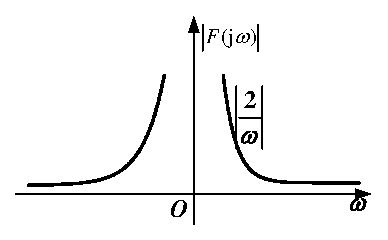
\includegraphics[width=30mm]{visio/4.10-a.pdf}
            \quad
        \end{FigureSub}
        \begin{FigureSub}[符号函数的相位频谱]
            \quad
            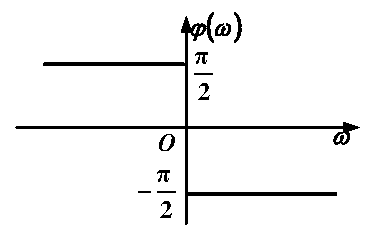
\includegraphics[width=30mm]{visio/4.10-b.pdf}
            \quad
        \end{FigureSub}
    \end{Figure}
\end{BoxFormula}

\begin{BoxFormula}[阶跃函数的傅里叶变换]
    阶跃函数满足
    \begin{Equation}
        \varepsilon(t) = \frac{1}{2} + \frac{1}{2}\mathrm{sgn}(t)
    \end{Equation}
    故其傅里叶变换为
    \begin{Equation}
        F(\mathrm{j}\omega) = \pi \delta(\omega) + \frac{1}{\mathrm{j}\omega}
    \end{Equation}
\end{BoxFormula}